\subsection{Introduction}\label{subsec:introduction_base_de_donnee}
Dans le contexte de mon application \("\)Clever Party Thrower\("\), une base de données est nécessaire pour gérer diverses informations générées par les utilisateurs,
ainsi que pour stocker d'autres données essentielles au bon fonctionnement de l'application.
Cette section fournit un aperçu détaillé de la conception, du choix, des opérations et de la structure de la base de données.

\subsection{Choix de la base de données}\label{subsec:choix-de-la-base-de-donnee}
Le choix du système de base de données est un aspect crucial de tout projet, car il influence directement les performances et la fonctionnalité de l'application.
Comme je l'ai précisé dans la section d'analyse, j'ai choisi un système de base de données de type SQL, plus précisément PostgreSQL, pour ce projet.
La haute disponibilité offerte par PostgreSQL, grâce à ses fonctionnalités avancées de réplication de données, a été l'une des principales motivations de ce choix.

De plus, PostgreSQL offre une grande extensibilité.
Son système d'extensions permet d'ajouter facilement des fonctionnalités à la base de données.
Par exemple, l'extension PostGIS, qui facilite le stockage et la manipulation des données géographiques, a été particulièrement utile pour mon application,
en particulier pour la fonction de covoiturage qui nécessite le calcul de la distance entre deux points géographiques.

En outre, le caractère open source de PostgreSQL, sa réputation solide et ses performances de haut niveau en font un choix idéal pour mon projet.
Sa compatibilité avec de nombreux langages de programmation et ORMs, dont TypeOrm que j'ai utilisé pour le développement de l'application, a consolidé ce choix.

\subsection{Opérations sur la base de données}\label{subsec:operation-sur-la-base-de-donnees}
Les opérations sur la base de données sont principalement de nature CRUD (Create, Read, Update, Delete).
Cependant, avec l'introduction du système de covoiturage, des opérations plus complexes sont devenues nécessaires.
Par exemple, le calcul des distances entre différents points géographiques est une opération essentielle pour la coordination du covoiturage.

\subsection{Structure de données}\label{subsec:structure-de-donnees}
La structure de la base de données est illustrée dans la figure ci-dessous.
Cette structure a été conçue pour garantir une exécution efficace des opérations de la base de données, tout en assurant la cohérence et l'intégrité des données.
Elle comporte plusieurs tables, dont chaque instance contient des informations pertinentes et est liée à d'autres tables pour créer des relations significatives entre les différentes données.
Voici une brève description ce chaque table de la basse de donnees
\begin{itemize}
    \item address : Contient des informations sur les adresses.
    Chaque instance d'adresse est liée à une instance de \("\) country \("\) (via \("\) countryId \("\)) et à une instance de \("\) user\_entity\("\) (via \("\)ownerId\("\)).
    \item car : Contient des informations sur les voitures.
    Chaque instance de voiture est liée à une instance de \("\)user\_entity\("\) (via \("\)ownerId\("\)).
    \item carpool : Contient des informations sur le covoiturage.
    \item Chaque instance de covoiturage est liée à une instance de \("\)address\("\) (via \("\)startPointId\("\) et \("\)endPointId\("\)), une instance de \("\)car\("\) (via \("\)carId\("\)),
    une instance de \("\)event\("\) (via \("\)eventId\("\)), et une instance de \("\)user\_entity\("\) (via \("\)driverId\("\)).
    \item country : Contient des informations sur les pays.
    Il est lié à \("\) address\("\) (via \("\)id\("\)).
    \item  dates\_t\_user : Contient des informations sur les dates liées aux utilisateurs.
    Chaque instance est liée à une instance de \("\)event\_date\("\) (via \("\) eventDateId\("\)) et à une instance de \("\)event\_to\_user\("\) (via \("\) eventToUserId\("\)).
    \item dept : Contient des informations sur les dettes.
    Chaque instance est liée à une instance de \("\)event\("\) (via \("\) eventId\("\)), et à deux instances de \("\) user\_entity \("\) (via \("\) creditorId\("\) et \("\)debtorId\("\)).
    \item event : Contient des informations sur les événements.
    Chaque instance est liée à une instance de \("\)address\("\) (via \("\)addressId\("\)) .
    \item event_date : Contient des informations sur les dates d'événement.
    Chaque instance est liée à une instance de \("\)event\("\) (via \("\)eventId\("\)).
    \item event_to_user : Contient des informations sur la relation entre les événements et les utilisateurs.
    Chaque instance est liée à une instance de \("\)address\("\) (via \("\)addressString\("\)), une instance de \("\)event\("\) (via \("\)eventId\("\)), et une instance de \("\)user\_entity\("\) (via \("\)userId\("\)).
    \item route_entity : Contient des informations sur les itinéraires.
    Chaque instance est liée à deux instances de \("\)address\("\) (via \("\)startingId\("\) et \("\)destinationId\("\)), une instance de \("\)carpool\("\) (via \("\)carpoolId\("\)), et une instance de \("\)user\_entity\("\) (via \("\)pickupId\("\)) .
    \item shopping_list_item : Contient des informations sur les articles de la liste de courses.
    Chaque instance est liée à une instance de \("\)event\("\) (via \("\) eventId\("\)) et à une instance de \("\)user\_entity\("\) (via \("\)assignedId\("\)).
    \item spending : Contient des informations sur les dépenses.
    Chaque instance est liée à une instance de \("\)event\("\) (via \("\)eventId\("\)), une instance de \("\)shopping\_list\_item\("\) (via \("\)shoppingListItemId\("\)), et une instance de \("\)user\_entity\("\) (via \("\)buyerId\("\)).
    \item user_entity : Contient des informations sur les utilisateurs.
    Chaque instance est liée à une instance de \("\)address\("\) (via \("\)addressId\("\)).
\end{itemize}

\begin{figure}[h!]
    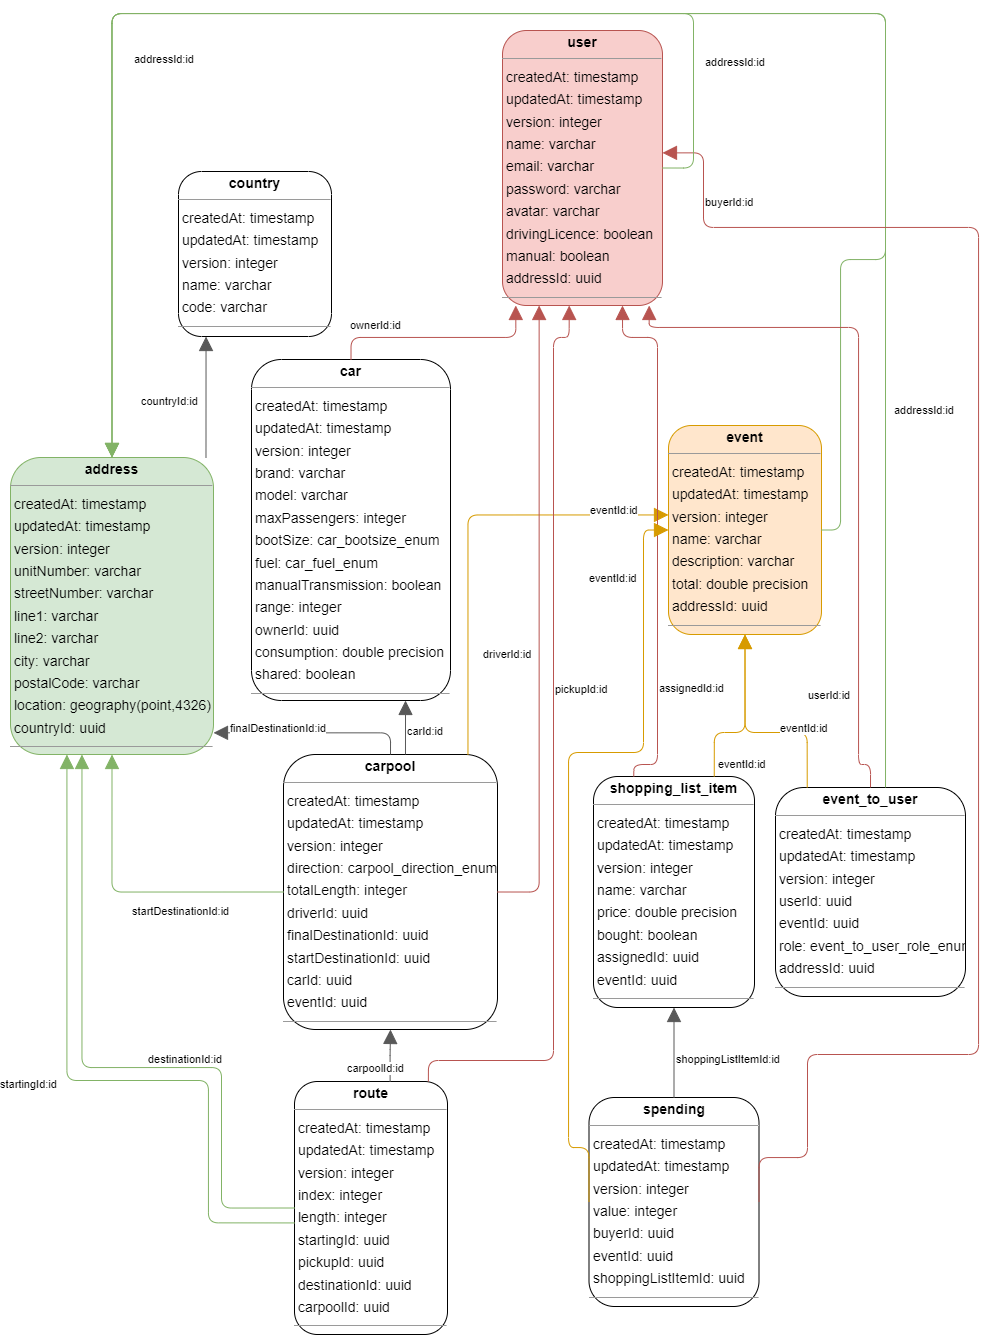
\includegraphics[width=\linewidth]{./images/dbShema}\caption{Architecture de la base de donnée}\label{fig:dbSchema2}
    \centering
\end{figure}